\newpage
\textcolor{red}{
    \subsection{TEXTO QUE PODE SER REAPROVEITADO}
    No modelo terceirizado, o provedor de identidade (ou servidor de autorização) emite credenciais específicas, conhecidas como Tokens de Acesso, para permitir que clientes terceiros obtenham acesso a recursos protegidos. Entretanto, esse método acarreta uma série de desafios, incluindo:
}
\textcolor{red}{   
    \begin{itemize}
        \item Falta de controle sobre credenciais: As credenciais criadas no ambiente online estão intrinsicamente ligadas aos provedores de identidade (\acs{IdP}), que têm o poder de revogar nosso acesso a elas. Isso implica que, se um usuário utilizar uma única credencial para múltiplos serviços e ela for revogada pelo \acs{IdP}, toda sua presença digital é comprometida, resultando na perda de acesso a esses serviços e possivelmente na perda de dados associados.
        \item Falta de autonomia sobre os atributos: Não há nenhum controle do que os \acs{IdP} podem fazer com os dados usuários, podendo utilizá-los sem o seu consentimento.
        \item Falta de privacidade: O \acs{IdP} conseguem monitorar todos os acessos dos usuários através do protocolo OAuth principalmente por meio do fluxo de autorização e dos tokens emitidos durante o processo de autenticação e autorização. 
    \end{itemize}
}


    Em contrapartida, o modelo \acs{SSI} resolve esses problemas concendo aos usuários um maior controle sobre seus dados pessoais e identidade online, que por sua vez, prejudica a experiência do usuário. Dessa forma, que o modelo proposto 
    
    
    Tradicionalmente, os protocolos de autenticação atuais pressupõem uma pressão sobre os usuários para que divulguem atributos de suas credenciais. Embora protocolos como OAuth tenham amenizado essa questão, eles transferem a responsabilidade de proteger os dados para o provedor de identidade. Isso é problemático, pois esses provedores podem não estar intrinsecamente comprometidos com a segurança dessas informações, como já discutido anteriormente. Neste contexto, o modelo fiduciário emerge como uma abordagem inovadora, distinguindo-se dos modelos existentes ao estabelecer um agente responsável que se compromete efetivamente a proteger as credenciais do usuário e autenticá-lo perante os provedores de serviço.

\newpage    
    \begin{lstlisting}[language=code, caption=Exemplo para a mensagem auth-response, label=input-label]
        {
            "from": "did:example:service-provider",
            "to": "did:example:fiduciary",
            "issuer": "did:example:issuer",
            "issuanceDate": "2018-11-27T12:37:15Z",
            "ZKProof": {
                "proof":
                {
                     "pi_a": [
                      "15054583087250400210539510268310299370352193228415727106012444162401960987255",
                      "8660045674621203434333353988056292866331758311663995238064641918875760339323",
                      "1"
                     ],
                     "pi_b": [
                      [
                       "20469564514415348581788554251320992722406997910387820030775419461195670848757",
                       "8226670483636230051887145511523069606491376738811303496825264018886389545639"
                      ],
                      [
                       "13775312170484599413218542585551322622526138169400293496163508841170235822115",
                       "7600889408431580307753477082245471784817027576450750926961372980721665697449"
                      ],
                      [
                       "1",
                       "0"
                      ]
                     ],
                     "pi_c": [
                      "9681129066519931648386919415389677386101432191842703087047602450490631444771",
                      "16540569009376506473468262707198528461836081711691615072411680586723972264887",
                      "1"
                     ],
                     "protocol": "groth16",
                     "curve": "bn128"
                }            
                "pubSignals": {
                     "0",
                     "19169662317894990683399855851481243806129670253992335137523572227625886599311",
                     "568080000",
                     "1711725073"
                } 
            }
        }
    \end{lstlisting}

\newpage
\section{PROTOCOLO}
\subsection{ALTO-NÍVEL}
\subsubsection{INTRODUÇÃO}

Esta especificação define um mecanismo sobre o modelo Fiduciário para solicitar e apresentar Apresentações Verificáveis com provas de zero-conhecimento. Como principal caraterística, o Protocolo Fiduciário permite os Usuários apresentarem Apresentações Verificáveis para Provedores de Serviço usando agente Fiduciário. 

Essas Apresentações Verificáveis com provas de zero-conhecimento são utilizadas pelo Fiduciário para demonstrar a posse de credenciais específicas contendo atributos particulares, sem, contudo, divulgar esses atributos.Por exemplo, um usuário (Beneficiário) pode acessar uma loja virtual de vinhos chilenos (Verificador) pela a intermediação do seu responsável (Fiduciário), sem revelar a sua idade para realizar sua compra.


Ademais, o protocolo Fiduciário também permite que os Provedores de Serviço solicitem mais informações sobre o usuário para a entidade Fiduciária. Essas requisições serão avaliadas conforme as políticas de consentimento já definidas e, caso de acordo, serão encaminhadas para a aplicação;.

Uma das grandes vantagens de adotar esse protocolo  é a liberdade que ele oferece aos programadores para tomarem suas próprias decisões em relação as tecnologias que poderam ser utilizadas. Isso inclui tipos de formatos de credenciais, sistemas de revogação, conjuntos criptográficos, e assim por diante.


Além disso, o protocolo tem a capacidade de permitir que o fiduciário negocie com o verificador o local onde a verificação da prova será executada. Nos modelos tradicionais, a verificação da correção de uma senha específica ou da validade de um token de autorização é realizada no lado do provedor de serviços. Ao direcionar essa verificação para um ambiente de confiança do usuário, o protocolo oferece uma vantagem significativa para o usuário. Isso possibilita que o processo de verificação ocorra em um ambiente no qual o usuário confie, beneficiando sua segurança e privacidade.


\subsubsection{PAPÉIS}

O protocolo define quatro papéis: 

\begin{itemize}
    \item Fiduciário: A entidade responsável por prover a autenticação do usuário para o provedor de servico. Ele tem acesso a credencial e por meio das politicas de consentimento define as melhores práticas de manipulação de dados
    \item Provedor de Serviço: Entidade que disponibiliza um serviço.
    \item Provedor de Identidade: Entidade responsável por emitir as credenciais do usuário.
    \item Usuário: Entidade capaz de garantir acesso a uma credencial
    \item Agente de usuário: Entidade intermediária entre um Usuário e o Provedor de Serviço. Ele envia solicitações HTTP para servidores web em nome do usuário, e recebe e exibe as respostas desses servidores. 
\end{itemize}

\subsubsection{TERMINOLOGIAS}
\begin{itemize}
    \item \textbf{Credencial Verificável}: É uma credencial que pode ser verificada criptograficamente por meio de tecnologias como assinaturas digitais. Essa definição é consoante ao \textbf{REF}
    \item \textbf{Apresentação Verificável}: Algumas dessas apresentações podem incluir provas de zero-conhecimento para gerar informações sobre os atributos contidos nas credenciais originais. Dessa forma, não é preciso conter as credenciais orginais, evitando exposição de dados desnecessária.
\end{itemize}



\subsubsection{VISÃO GERAL}

Abaixo estão definidos os dois fluxos possíveis dentro do protocolo. O primeiro é o diagrama de fluxo em que o Fiduciário identifica seu usuário através uma Apresentação Verificável a um Provedor de Serviço. O segundo, é o digrama de fluxo em que o Provedor de Serviço precisa de mais informações sobre o usuário. \\ \\


\begin{figure}[h]
    \centering
    \includegraphics[scale=0.5]{images/protocolo_fiduciario_identificaçao.png}
    \caption{Fluxo de mensagem para identificação do usuário.}
    \label{fig:fluxo-identity}
\end{figure}

\begin{enumerate}
    \item O \acs{SP} inicia o processo enviando uma solicitação de identificação ao Fiduciário (\textit{\textbf{identity-request)}}. Esta solicitação inclui uma definição de apresentação no campo \textit{\textbf{presentation\_definition}}, a qual descreve os requisitos dos atributos das Credenciais que o \acs{SP} deseja. Esses requisitos podem abranger quais emissores são confiáveis, quais algoritmos de zero-conhecimento são aceitáveis, quais informações precisam ser divulgadas, entre outros critérios. 
    
    \item O Fiduciário solicita a autenticação do usuário por meio de seu Agente de Usuário, o qual a responde com suas informações necessárias. Em seguida, o Fiduciário  processa a Solicitação de Autenticação com a definição de Apresentação Verificável, determinando quais Credenciais necessárias para gerá-la à solicitação do \acs{SP}.
    
    \item O Fiduciário prepara a Apresentação à qual o Usuário  consentiu por meio de suas políticas já definidas. Em seguida, o Fiduciário envia ao \acs{SP} uma Resposta de Identificação (\textbf{\textit{identity-response}}) onde a Apresentação Verificável está contida no parâmetro \textbf{\textit{vp}}.

\end{enumerate}

Se o Provedor de Serviços necessitar de informações adicionais sobre o usuário ele pode utilizar o segundo fluxo de aquisição de informação. Para isso, ele deve enviar uma mensagem de solicitação de informações, denominada \textbf{\textit{identity\_request\_info}}, contendo o \textbf{\textit{token\_userdetails}} para o \textit{endpoint} \textit{\textbf{/identityinfo}}. Esta mensagem deverá incluir o parâmetro \textbf{\textit{presentation\_definition}} (ou \textit{presentation\_definition\_url}). Posteriormente, ela será processada e analisada de acordo com as políticas de consentimento. Se estiver em conformidade com tais políticas, será gerada uma Apresentação Verificável adicional contendo as informações solicitadas ou a comprovação de que o usuário detém tais informações. Por exemplo, um \acs{SP} pode solicitar a idade do usuário para permitir a compra de bebidas alcoólicas, porém, se a política do usuário não permitir o compartilhamento dessa informação, o fiduciário poderá gerar uma prova de conhecimento zero. Essa prova irá confirmar duas coisas: primeiramente, que o usuário possui uma credencial válida que inclui sua idade; e em segundo lugar, que a idade do usuário é igual ou superior à idade mínima requerida para a compra de bebidas alcoólicas no contexto em questão. \\ \\\

\begin{figure}[h]
    \centering
    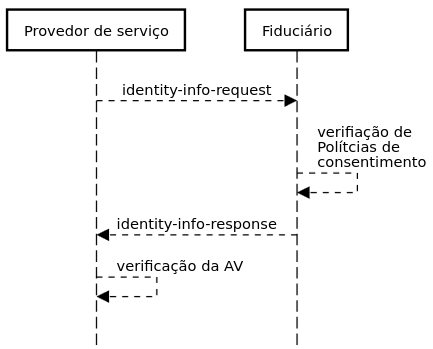
\includegraphics[scale=0.5]{images/protocolo_fiduciario_info.png}
    \caption{Fluxo de mensagem para conseguir informações do usuário.}
    \label{fig:fluxo-info}
\end{figure}

\begin{enumerate}
    \item O \acs{SP} inicia o processo enviando uma solicitação de informações ao Fiduciário (\textit{\textbf{identity-info-request)}}. Esta solicitação também inclui uma definição de apresentação no campo \textit{\textbf{presentation\_definition}}, a qual descreve os requisitos dos atributos das Credenciais que o \acs{SP} deseja.
    
    \item O Fiduciário verifica se o \textbf{\textit{token userdetails}} é válido, obersando sua data de emissão, validação e se ele foi emitido pelo Fiduciário. Em caso positivo de \textit{token} ser válido e as informações estiverem de acordo com as políticas de consentimento, o Fiduciário prepara a Apresentação Verificável e  envia ao \acs{SP} uma resposta de informação (\textbf{\textit{identity-info-response}}) onde a Apresentação Verificável está contida no parâmetro \textbf{\textit{vp}}.

\end{enumerate}

\subsection{MENSAGEM DE REQUISIÇÃO DE SERVIÇO}

Nesta mensagem, é explicado o tipo de serviço solicitado, o qual varia de acordo com a implementação do provedor de serviço (SP). É essencial que o usuário informe a URL do seu fiduciário como requisito obrigatório. Essa URL é necessária porque como não estamos exigindindo nenhuma etapa de registro prévia, como acontece nos outros protocolos como OAuth e OIDC em que um \textit{client\_id} e um \textit{client\_secret} são estabelecidos entre o provedor de serviços e o servidor de autorização. Dessa forma, o \ac{SP} precisa da URL para redirecionar o usuário para seu agente fiduciário.


\subsection{MENSAGEM DE REQUISIÇÃO DE IDENTIFICAÇÃO}

Nesta mensagem enviada pelo \acs{SP} ao Fiduciário, são especificados os requisitos para identificar o usuário. O Fiduciário tem a obrigação de criar uma prova de conhecimento zero e incluí-la na resposta de identificação, possibilitando ao usuário utilizar o recurso. Nessa mensagem apenas dois, para parâmetros são necessários: presentation\_definition, ou por valor ou referência, e o \textit{nonce}.

\begin{itemize}
    \item \textbf{presentation\_definition:} Campo OBRIGATÓRIO que contém um objeto JSON de Definição de Apresentação. Este parâmetro DEVE estar presente quando o parâmetro presentation\_definition\_uri não estiver presente.


    \item \textbf{presentation\_definition\_uri}: Campo OBRIGATÓRIO que contém um URL HTTPS apontando para um recurso onde um objeto JSON de Definição de Apresentação pode ser recuperado. Este parâmetro DEVE estar presente quando o parâmetro presentation\_definition não estiver presente.

    \item \textbf{nonce}: Campo OBRIGATÓRIO que ajuda a prevenir ataques de repetição, garantindo que cada solicitação seja tratada como única, por meio da vinculação das Apresentações Verificáveis ao contexto da transação em que estão sendo usadas.
\end{itemize}


Um exemplo de mensagem de Identificação é mostrada a seguir:

\begin{lstlisting}[language=code, caption=Exemplo para a mensagem id-request, label=input-label]
    GET /identify?
    &presentation_definition=...
    &nonce=n_1D7_ExS3Nk HTTP/1.1
\end{lstlisting}


\subsection{MENSAGEM DE RESPOSTA DE IDENTIFICAÇÃO}

O sistema SP usa o parâmetro \textbf{\textit{presentation\_definition}} ou \textit{\textbf{presentation\_definitin\_uri}}, os quais apresentam o JSON que descreve a definição para a Credencial solicitada. Isso inclui um. O Fiduciário deve examinar esse JSON e escolher a Credencial Verificável apropriada.

\begin{itemize}
    \item \textbf{vp}: Campo OBRIGATÓRIO com apenas uma Apresentação Verificável ou uma lista de Apresentações Verificáveis sendo cada uma das Apresentação Verificável deve ser representada um objeto JSON. 
    
    \item \textbf{presentation\_submission}: Campo OBRIGATÓRIO definido em [] que organiza informações sobre as credenciais que foram requisitadas e onde encontrá-las dentro das Apresentaçõeos Verificáveis mandadas em \textit{vp}.

    \item \textbf{token\_userdetails}: Campo OBRIGATÓRIO que contém um token encaminhado pelo Fiduciário ao \acs{SP} para que ele possa requisitar informações sobre um determinado usuário. Ele deve ser encaminhado sempre para o endpoint \textit{/identityinfo}.

    \item \textbf{issuer\_identifier}: Campo OBRIGATÓRIO que identifica o Provedor de Identidade utilizado para assinar a credencial do usuário. 
    
    
    \item \textbf{issuer\_public\_key}: Campo OBRIGATÓRIO que onde recuperar a chave pública utilizada pelo o Provedor de Identidade utilizada para assinar a credencial do usuário. 

\end{itemize}

\begin{lstlisting}[language=code, caption=Exemplo para a mensagem id-response, label=input-label]
  HTTP/1.1 302 Found
  Location: https://fiduciary.com/cb#
    presentation_submission=...
    &vp=...
    &token_userdetails=...
    &issuer_identifier=...
    &issuer_public_key=...
\end{lstlisting}

\subsection{MENSAGEM DE RESPOSTA DE SERVIÇO}

Esta mensagem é a resposta se o \acs{SP} aceitou ou não a identificação do usuário.

\section{Token userdetails}

É um token usado pelos \acs{SP} para requisitar mais informções sobre o usuário que está acessando seu serviço. Deve ser encaminhado no endpoint \textit{/identityinfo} do respectivo fiduciário. O Fiduciário ao receber esse token deve avaliar se tal pedido segue a políticas de consentimento definidas pelo o seu usuário. Caso positivo, encaminha uma resposta para \acs{SP} com as informações do usuário sobre um canal seguro. Caso negativo, o fiduciário encaminha uma mensagem que contém uma lista de sugestões de atributos os quais o seu usuário concede de maneira pública sobre determinadas condições.



\subsection{FLUXO 1: Fiduciário realiza a geração de prova}
\subsection{FLUXO 2: Verificador realiza a geração de prova}

\subsection{FLUXO IMPLÍCITO DO OAUTH}

A principal diferença entre este fluxo e o descrito anteriormente está na obtenção e transmissão dos tokens entre as partes envolvidas. No fluxo implícito, os tokens de acesso são transmitidos diretamente para o aplicativo cliente no momento da autorização, em vez de passarem por um código de autorização intermediário. Após a autenticação do usuário, o Servidor de Autorização redireciona o usuário de volta para a aplicação com o token de acesso incluído na resposta.

Devido à ausência de uma troca explícita de código de autorização e à entrega direta dos tokens de acesso ao aplicativo (no frontend), este fluxo é menos seguro. Os tokens de acesso ficam expostos no navegador do usuário, o que aumenta o risco de serem interceptados por atacantes.